%!TEX root = ../thesis.tex
%*******************************************************************************
%*********************************** First Chapter *****************************
%*******************************************************************************


\chapter{Introduction and literature review}


\ifpdf
    \graphicspath{{Chapter1/Figs/Raster/}{Chapter1/Figs/PDF/}{Chapter1/Figs/}}
\else
    \graphicspath{{Chapter1/Figs/Vector/}{Chapter1/Figs/}}
\fi

%*******************************************************************************


\section[Motivation for research and historical background]{Motivation for research and historical background}
\label{section1.1}

\todo{Make bib file and convert these reeferences to correct format}

\subsection[History of early modern English wall paintings]{History of early modern English vernacular wall paintings}
\label{subsection1.1.1}

\todo{LOLLLLLL this needs to be written.}

\subsection[Open research questions about wall paintings]{Open research questions about wall paintings and early modern material culture}
\label{subsection1.1.2}

While there are many aspects of early modern material culture that are not well understood today, including the extent and significance of wall paintings created in the early modern period, this research is concerned with the open questions relating to the materiality of these works. There has been limited research into the materials used by craftsmen due to the difficulty of carrying out scientific analysis on a large number of samples.~\cite{baird,davies} The availability of various blue (and, to a lesser extent, green) pigments during this period has been subject to debate, and the language used to describe blue pigments has been inconsistent and scientifically inaccurate.~\cite{harley} 

In particular, the use of synthetic copper carbonate blue pigments (blue verditer) has been noted anecdotally in Suffolk.~\cite{baird, others you need to find} This discovery must be confirmed and a larger body of samples should be analyzed to determine the extent of use. This is significant to the interpretation of vernacular wall paintings, particularly their purpose, cost, value to homeowner, and disposability.~\cite{baird,davies} Additionally, the availability of synthetically produced pigments to the middling class could indicate new industrial methods of production and close ties between scientists and the artists and craftsmen who they supplied. 

This work also has important implications for preservation and restoration of these works, which are often in poor condition or at risk of being lost entirely. Many vernacular wall paintings from this period exist in the historical record but have since been demolished, although experts on early modern material culture maintain their importance to our understanding of daily life during the period.~\cite{davies,a day at home,benton 1, benton 2} Azurite and verditer pigments are unstable and can be altered by excessive humidity and alkalinity, as well as light exposure, and this research could inform future preservation and restoration choices made about these important works.~\cite{humidity paper, alkalinity paper, degradation products paper, light needs a reference}

\section[Research plan and scientific background]{Research plan and scientific background}
\label{section1.2}

\subsection[Plan for sampling and analysis]{Plan for sampling and analysis}
\label{subsection1.2.1}

\todo{Reiterate: unanswered questions are primarily 1) the identity of pigments used in wall paintings in Suffolk (XXXX check, how big range of sampling is) and 2) the method of production of these pigments, including the determination of viability of synthetic recipes from the time.

Note methods that we intend to use (AFM IR, Raman, SEM-EDS, microscopy..?). What information these will give, and how this information will be useful in answering the above questions.

Explain samples that will be analysed- the sources, locations, why these were selected. This cannot be completed yet, but the reference samples can be discussed at this point.}

\subsection[Previous work on copper carbonate pigments]{Previous work on copper carbonate pigments}
\label{subsection1.2.2}

Previous work has characterised azurite and malachite and degradation products thereof using confocal Raman spectroscopy and infrared specroscopy. The use of and production of synthetic blue and green pigments in England and continental Europe has been minimally studied. Additionally, synthetic recipes from the medieval period have been evaluated for their success in producing pigments.

Frost et. al. have studied malachite and azurite using confocal and polarised Raman spectroscopy, giving a clear explanation of peak assignments and determining that these minerals do show orientation dependence in their spectra.~\cite{frost} Bicchieri et. al. used micro-Raman and laser indused breakdown spectroscopies to study lapis lazuli and azurite pigments on parchment.~\cite{bicchieri} 

Saunders et. al. have studied the changes azurite undergoes upon exposure to high humidity, noting that azurite has been observed to degrade to malachite or green copper chlorides under various environmental conditions. They found that azurite was largely unaffected by light under all humidity conditions, with one sample forming copper chlorides in the presence of NaCl and one inexplicably darkening.~\cite{saunders} Cardell et. al., on the other hand, determined that azurite was altered by natural (outdoor) and artificial ultraviolet light exposure, showing that effects were dependent on pigment grain size.~\cite{cardell} Lluveras et. al. mapped green degradation products using synchrotron radiation, determining that copper oxalates and copper hydroxychlorides formed in different areas of the azurite surface depending on proximity to calcium and chlorine ions respectively.~\cite{lluveras} The chemical heterogeneity observed here supports the use of surface analytic techniques such as AFM-IR. 

Mattei et. al. addressed the degradation of azurite induced by exposure to heat and exposure to alkaline conditions. They note that azurite is not very stable, degrading easily to form malachite, to Cu2Cl(OH)3 (atacamite, paratacamite or clinoatacamite), or less often to CuS or CuO (tenorite). They note a green inclusion present in azurite samples that was not malachite or a yellow iron oxide. Tenorite was found following heating of azurite particles, and degradation is dependent on the size of the pigment grain. Tenorite was also found following exposure to alkaline terra cotta. Beyond this, however, they did not discuss alterations to crystal structure and did not measure the depth of penetration into the sample.~\cite{mattei} 

Naumova et. al. have studied the green pigments used in medieval Russian frescoes dating to the 1500s, and have identified several synthetic pigments for which recipes from the period are not known. They note that artificial pigments were typically circular in grain shape and showed a characteristic black cross when viewed under a polarised microscope through crossed nicol prisms. However, these identifiers are noted in the same work to be problematic and inaccurate at times. Naumova et. al. also attempted to recreate historic recipes for blue and green pigments, and were unable to synthetically produce azurite. This is one of few sources that does discuss the use of synthetic pigments, and concludes that further research is necessary in this area.~\cite{naumova 1, naumova 2}

Orna et. al. have discussed and evaluated medieval recipes claiming to produce blue pigment from the treatment of silver and copper metals. Treatment of copper containing alloys with acetic acid under different heating conditions formed verdigris and copper acetate, but copper carbonates were not observed.~\cite{orna 1, orna 2} Seldes et. al. identified azurite in several fine art works from South America painted during the 1700s, and determined that the pigment was referred to by Spanish artists as ``blue powder" or ``blue ashes." 

MacTaggart et. al. studied recipes for producing blue and green verditer, which are the synthetic analogues of azurite and malachite. Blue verditer is also referred to as ``blue bice" and ``blue ashes." They discuss previously identified characteristics of historic verditers, ``tiny, rounded, fibrous aggregates, even in size, highly birefracting, and blue by transmitted light." There are credible historical references to verditers dating to the early 1500s, and they claim that blue verditer was a speciality of English producers at this time. One challenge, however, is that the authors note that blue verditer was also used as a general term to refer to any blue pigments at the time regardless of composition or production. In order to determine a successful method for producing verditers that meet previously identified physical markers, they tested the procedure for refining gold for which blue verditer was a byproduct. Ultimately, they struggled to produce blue verditer consistently, as did early modern refiners, and they proposed that the success or failure of synthesis was dependent on the weather; blue particles are only produced at temperatures below 12 \textdegree C.~\cite{mactaggart}

Aru et. al. have characterised the mineral impurities present in many samples of azurite from source mines known in the medieval period using Raman spectroscopy. Many minerals were discovered as natural inclusions in most samples, including malachite, hematite, goethite, cuprite, and titanium dioxides. Others were less common, such as quartz, calcite, cerussite, orthoclase, beudantite and jarosite. Tenorite, identified by XXXX et. al. as a degradation product of azurite, was not identified as an impurity in these samples. Unfortunately, though the samples were collected from mines that were active during the medieval period, they dated at the earliest to the eighteenth century, and the small sample size precludes the use of impurities to conclusively trace provenance of azurite samples.~\cite{aru} However, this research does suggest that the presence of trace minerals in natural samples is indicative of environmental conditions when azurite crystals form, and that these minerals should be studied in a larger sample set to determine whether any patterns in their occurrence can be identified. This supports the use of techniques that detect surface heterogeneity and suggests that mineral inclusions may differ in natural versus artificial samples.

XXXX Remaining to do: All the things I havent read yet!!!

\section[Methodology and theoretical background]{Methodology and theoretical background}
\label{section1.2}

Raman, SEM, EDS, AFM-IR.. etc
Raman and AFM-IR sections are from MPhil thesis and must be revised.

\subsection[Confocal Raman spectroscopy]{Confocal Raman spectroscopy}
\label{subsection1.2.2}

The basis of Raman spectroscopy is the interaction between photons from an incident laser beam and molecules or particles in the sample. Photons with a known energy $E_{in} = h\nu$ are scattered off the sample surface. The majority of these  photons return from the sample at the same energy due to elastic collisions, a process known as Rayleigh scattering. A small percentage of photons are inelastically scattered, and return at either higher or lower energies than the incident beam. Most commonly, they lose energy, with 

\begin{equation} \label{eq:raman_1}
E_{out} = E_{in} - \Delta E
\end{equation}

where $E_{out}$ is the energy of the photon emitted from the sample. This is known as Stokes scattering. The other case is known as Anti-Stokes scattering. Stokes scattering is more common since most molecules in the sample are in their ground vibrational state at room temperature and therefore cannot transfer vibrational energy to the incident photon. The change in energy $\Delta E$ depends on the vibrational levels of the sample:

\begin{equation} \label{eq:raman_2}
\Delta E = E_{ex} - E_{g}
\end{equation}

where $E_{g}$ is the energy of the ground vibrational state and $E_{ex}$ is the energy of the excited vibrational state. Different bonds have different vibrational modes and thus different Raman shifts, which makes this technique useful in identifying samples since each different molecule or compound produces a characteristic Raman spectrum.~\autocite{2018RS,horiba,matousek_tissue} Raman shifts also shed light on chemical and structural changes in a sample. Peak broadening and shifts indicate changing chemical environments, while relative peak intensities indicate different degrees of disorder or loss of certain bonds.~\autocite{tomasini_raman}

Although Raman and infrared spectroscopy operate on similar principles of light interacting with samples and perturbing their vibrational modes, the way they work is different and therefore there are different selection rules for each method. Infrared spectroscopy involves the absorption of incident energy by the sample, leading to a change in vibrational energy level. Only vibrational modes that involve a change in the overall dipole moment of the molecule are IR active, so this method cannot be used to investigate symmetric vibrational modes with inversion centres.~\autocite{hashimoto} Raman spectroscopy, on the other hand, requires a change in the polarisability or transient dipole of the molecule, so symmetric modes are Raman active.~\autocite{2018RS,inphotonics}

\subsection[Atomic force microscopy]{Atomic force microscopy}
\label{subsection1.2.2}

Atomic force microscopy works by using a very narrow and sharp physical probe attached to a flexible cantilever to investigate sample properties. This method has a significant advantage compared to traditional light microscopy which is limited by an inherent diffraction limit of $\lambda$/2 for incident light with wavelength $\lambda$. This is typically on the order of several hundred nanometers to several microns. AFM, on the other hand, can achieve resolution of below 20 nm, which allows better visualisation of chemical heterogeneity.~\autocite{dazzi2017} 

Interactions between the AFM tip and the surface cause the cantilever to be deflected and oscillate like a spring. This oscillation is detected by a laser that illuminates the cantilever and is reflected into a photodiode detector. AFM images can be collected in tapping mode, where the tip is brought into and out of contact with the surface, or contact mode, where the tip drags along the surface. In contact mode, a topography or height map can be generated from a surface. Additionally, changes in frictional forces on the surface can be measured by the side-to-side deflection of the tip as it moves in contact mode.~\autocite{friction_afm} 

Conventional infrared spectroscopy, as it also relies on light interacting with a sample, is diffraction limited. AFM-IR offers far superior resolution because the infrared signal is produced by measuring the infrared-induced thermal expansion of the sample using the tip and is therefore limited by the size of the tip radius.~\autocite{dazzi2017,kurouski} \textit{Figure \ref{fig:afm_diagram}} shows a schematic diagram of the detection of infrared spectra using an AFM. 

\begin{figure}[H]
\centering
  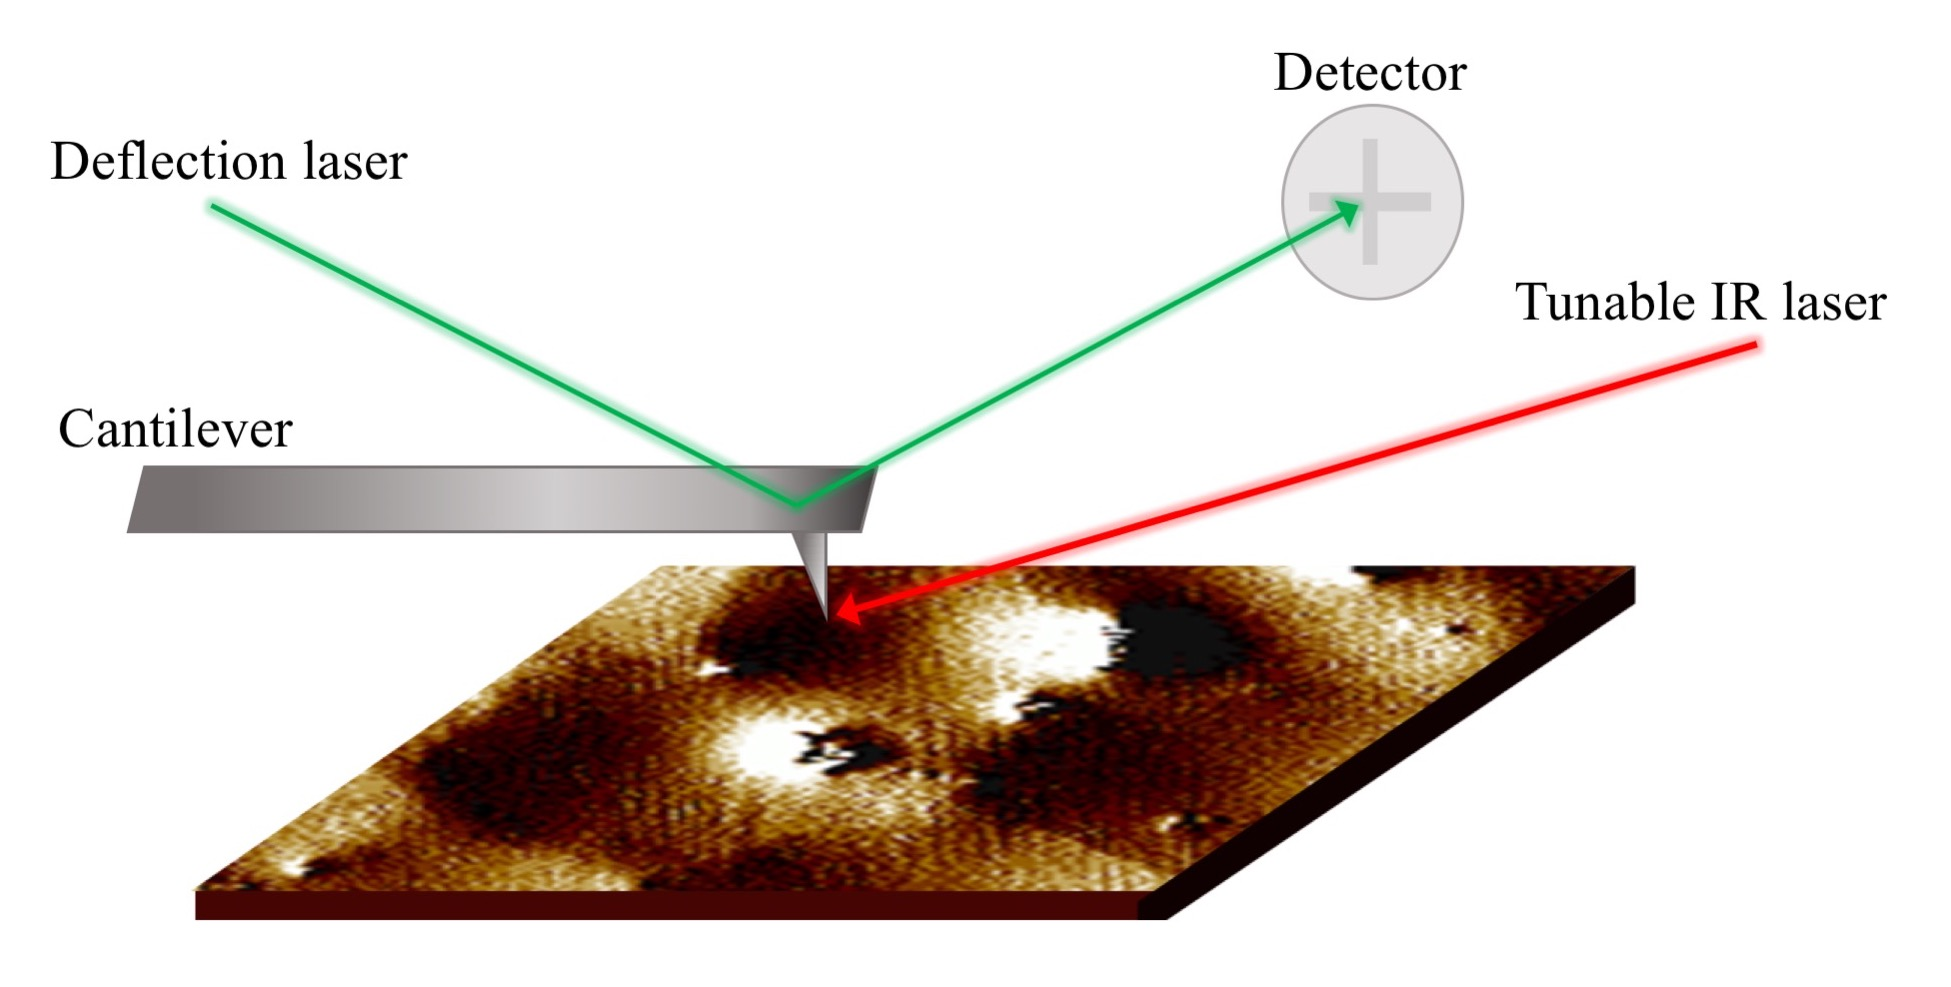
\includegraphics[width=\linewidth]{afm_diagram}
\caption[Diagram of AFM-IR schematic showing a top-down illumination system.]{Diagram of AFM-IR schematic showing a top-down illumination system. The incident infrared beam is absorbed by the sample and the resulting thermal expansion causes the tip and cantilever to move. This cantilever deflection is registered by another laser whose beam is detected by a photodiode.~\autocite{Morsch,dazzi2017}}
\label{fig:afm_diagram}
\end{figure}

The thermal expansion of the sample upon absorption of infrared light imparts a force to the tip and this induces oscillations in the cantilever. Dazzi et. al. have shown that the cantilever oscillations are proportional to the absorption coefficient of the sample, which is important since this enables direct comparison of AFM-IR and conventional transmittance IR spectra (i.e., band shapes and locations are not changed by the method of collection).~\autocite{dazzi2017,kurouski} 

Spectra can be collected either by scanning over a range of infrared frequencies at a single location or over a range of locations on the sample at a single infrared frequency (infrared mapping).~\autocite{dazzi2017,kurouski} While there are some downsides to this technique such as long sampling times and increased sensitivity to background shifts compared to conventional infrared spectroscopy, it is an exciting novel technique for nanoscale surface studies.

\subsection[Scanning electron microscopy]{Scanning electron microscopy}
\label{subsection1.2.2}

 \todo{Needs writing.}



